\documentclass[11pt]{article}
\usepackage[utf8]{inputenc}
\usepackage[T1]{fontenc}
\usepackage{amsmath}
\usepackage{amsfonts}
\usepackage{amssymb}
\usepackage[version=4]{mhchem}
\usepackage{stmaryrd}
\usepackage{graphicx}
\usepackage[export]{adjustbox}
\graphicspath{ {./images/} }

\begin{document}
\section*{Reading}
Option Pricing Models

Modern option pricing models are precise tools with applications that permeate investment analysis, especially alternative investment analysis. This section provides a somewhat nontraditional view of continuous time option-pricing models, starting with the generalized case of an exchange option rather than with the classic Black-Scholes call option pricing model. ${ }^{1}$ William Margrabe, "The Value of an Option to Exchange One Asset for Another," Journal of Finance 33, no. 1 (1978): 177-86. Throughout the analysis, it is assumed that the underlying asset does not pay any cash distributions.

\section*{FOUNDATION CHECK}
This section assumes basic familiarity with applying the Black-Scholes option pricing model, including application of the cumulative normal distribution.

\section*{An Option on a Portfolio}
Most option pricing models can be shown as special cases of the simple model introduced in Equation 1. Consider a portfolio that has both one or more long positions and one or more short positions, with a current net market value that may be positive or negative. An investor has an option either to take ownership of both sides of the portfolio or to walk away from the transaction and let the option expire at some fixed expiration date. The value for the option on this portfolio is given by this simple equation: ${ }^{2}$ Compared to most option pricing models!

\begin{center}

\includegraphics[max width=\textwidth]{2024_04_11_7c728ae44168a8fb26cag-2(1)}
\end{center}


\begin{equation*}
P_{o}=P_{l} N(d)-P_{s} N(d-v) \tag{1}
\end{equation*}


where $P_{o}=$ the value of the option, $P_{l}=$ the value of the long positions, $P_{s}=$ the value of the short positions, $N(\cdot)=$ the cumulative normal distribution, $d=\left[\ln \left(P_{l} / P_{s}\right) / v\right]+(v / 2)$, and $v=$ the return volatility of the portfolio integrated over the time to expiration.

Note that the relevant measure of volatility, $v$, is based on the volatility of the combined long and short positions. The volatility of the portfolio is therefore based on the volatility of the long positions, the volatility of the short positions, and the correlation between the two positions.

The distinction between calls and puts is simplified by viewing this generalized case. A call option is when the short position is a fixed cash flow (i.e., a zero-coupon bond), and a put option is when the long position is a fixed cash flow. If both positions are fixed cash flows, denominated in different currencies, then Equation 1 becomes an FX (foreign exchange) or currency option.

\section*{The Black-Scholes Call and Put Option Formulae}
As indicated previously, a call option is the special case of Equation 1 in which the long position is an asset, such as a share of common stock, say $S$, and the short position is a zero-coupon bond with a face value of $K$ that matures when the option expires. Substituting into Equation 1 produces the famous Black-Scholes (1973) call-option formula (continuing to assume no dividends) for the price of a call. ${ }^{3}$ Fischer Black and Myron Scholes, "The Pricing of Options and Corporate Liabilities," Journal of Political Economy 81, no. 3 (1973): 637-54. The Black-Scholes call option formula expresses the price of a call option as a function of five variables: the price of the underlying asset, the strike price, the return volatility of the underlying asset, the time to the option's expiration, and the riskless rate, as shown in Equation 2:

\begin{center}
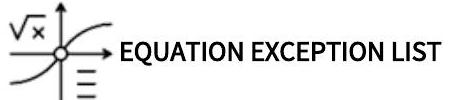
\includegraphics[max width=\textwidth]{2024_04_11_7c728ae44168a8fb26cag-2}
\end{center}

$$
\begin{aligned}
c & =S N\left(d_{1}\right)-e^{-r T} K N\left(d_{2}\right) \\
d_{1} & =\left[\ln \left(S / e^{-r T} K\right) / v\right]+(v / 2) \\
d_{2} & =d_{1}-v \\
v & =\sigma_{s} \sqrt{T}
\end{aligned}
$$

where $c$ is the call option price, $r$ is the riskless rate, $T$ is the time to the option's expiration, and $\sigma_{s}$ is the constant volatility of the returns of $S$. The Black-Scholes model assumes that the riskless rate and the volatility of the stock, $\sigma_{s}$, are constants. The constant volatility assumption and the absence of correlation between the stock price and the strike price simplify $v$ to being $K$. If the short position is an asset, such as a share of common stock, and the long position is a zero-coupon bond with a face value of $K$ that matures when the option expires, then Equation 1, with some rearrangement, is the familiar Black-Scholes put option formula.

\section*{The Black Forward Option Pricing Model}
Black (1976) derived an option pricing model for a call option on a forward contract: ${ }^{4}$ Fischer Black, "The Pricing of Commodity Contracts," Journal of Financial Economics 3, no. 1/2 (January/March 1976): 167-79.

\begin{center}
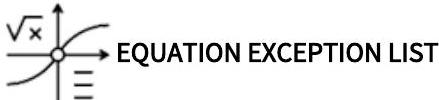
\includegraphics[max width=\textwidth]{2024_04_11_7c728ae44168a8fb26cag-3}
\end{center}

$c=e^{-r T}\left[F N\left(d_{1}\right)-K N\left(d_{2}\right)\right]$

$d_{1}=[\ln (F / K) / v]+(v / 2)$

(3)

$d_{2}=d_{1}-v$

where $F$ is the forward price. Note that the model is easily derived from the Black-Scholes formula by substituting for $S$ from the cost-of-carry model in the Forward Contracts on Assets with Benefits and Costs of Carry lesson.: $S=e^{-(r-d) T} F(T)$, and setting the dividend yield to zero. It should be noted that $e^{-r T}$ vanishes from $d_{1}$ in the case of an option on a forward. The intuition of the model is that since neither the forward contract nor the strike price requires an initial investment, both variables need to be discounted, so $r$ drops out of the model.

\section*{The Currency Option Pricing Model}
A currency option pricing model was derived by Biger and Hull (1983). ${ }^{5}$ Nahum Biger and John Hull, "The Valuation of Currency Options," Financial Management 12 (1983): 24-28. The distinguishing feature of the currency or currency exchange model is that there are two riskless interest rates corresponding to the two currencies being exchanged:

\begin{center}
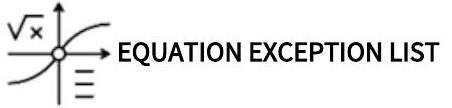
\includegraphics[max width=\textwidth]{2024_04_11_7c728ae44168a8fb26cag-3(1)}
\end{center}

Option Price $=e^{-r^{*} T} S^{*} N\left(d_{1}\right)-e^{-r T} S N\left(d_{2}\right)$

Equation 4 is an option to exchange $S^{\star}$ units of one currency with an associated riskless interest rate of $r^{\star}$ for $S$ units of another currency with an associated riskless interest rate of $r$. Both interest rates also appear in the formula for $d_{1}$ in the case of a currency exchange option.


\end{document}